% !TEX TS-program = xelatex
\documentclass[10pt,landscape,a4paper]{article}
%\usepackage[utf8]{inputenc}
%\usepackage[ngerman]{babel}
\usepackage{tikz}
\usetikzlibrary{shapes,positioning,arrows,fit,calc,graphs,graphs.standard}
\usepackage[nosf]{kpfonts}
\usepackage[t1]{sourcesanspro}
%\usepackage[lf]{MyriadPro}
%\usepackage[lf,minionint]{MinionPro}
\usepackage{multicol}
\usepackage{wrapfig}
\usepackage[top=0mm,bottom=1mm,left=0mm,right=1mm]{geometry}
\usepackage[framemethod=tikz]{mdframed}
\usepackage{microtype}
%\usepackage{physics}
\usepackage[font=scriptsize]{caption}
\usepackage{tabularx}
\usepackage{hhline}
\usepackage{makecell}
\usepackage{mathtools}
\DeclarePairedDelimiter{\ceil}{\lceil}{\rceil}

\newcommand\codeblue[1]{\textcolor{blue}{\code{#1}}}

\usepackage{lastpage}
\usepackage{datetime}
\yyyymmdddate
\renewcommand{\dateseparator}{-}
\let\bar\overline

\definecolor{myblue}{cmyk}{1,.72,0,.38}

\def\firstcircle{(0,0) circle (1.5cm)}
\def\secondcircle{(0:2cm) circle (1.5cm)}

\colorlet{circle edge}{myblue}
\colorlet{circle area}{myblue!5}

\tikzset{filled/.style={fill=circle area, draw=circle edge, thick},
    outline/.style={draw=circle edge, thick}}

\pgfdeclarelayer{background}
\pgfsetlayers{background,main}

%\everymath\expandafter{\the\everymath \color{myblue}}
%\everydisplay\expandafter{\the\everydisplay \color{myblue}}


\renewcommand{\baselinestretch}{.8}
\pagestyle{empty}

\global\mdfdefinestyle{header}{%
linecolor=gray,linewidth=1pt,%
leftmargin=0mm,rightmargin=0mm,skipbelow=0mm,skipabove=0mm,
}

\newcommand{\header}{
\begin{mdframed}[style=header]
\footnotesize
\sffamily
CS2030 Finals Cheatsheet v1.0\\(\today)\\
by~Julius Putra Tanu Setiaji,~page~\thepage~of~\pageref{LastPage}
\end{mdframed}
}
%\usepackage{chngcntr}

\usepackage{verbatim}

\usepackage{etoolbox}
\makeatletter
\preto{\@verbatim}{\topsep=0pt \partopsep=0pt }
\makeatother

\counterwithin*{equation}{section}
\counterwithin*{equation}{subsection}
\usepackage{enumitem}
\newlist{legal}{enumerate}{10}
\setlist[legal]{label*=\arabic*.,leftmargin=2.5mm}
\setlist[itemize]{leftmargin=2.5mm}
\setlist[enumerate]{leftmargin=3.5mm}
\setlist{nosep}
\usepackage{minted}

\def\code#1{\texttt{#1}}

\newenvironment{descitemize} % a mixture of description and itemize
{\begin{description}[leftmargin=*,before=\let\makelabel\descitemlabel]}
  {\end{description}}

\newcommand{\descitemlabel}[1]{%
  \textbullet\ \textbf{#1}%
}
\makeatletter



\renewcommand{\section}{\@startsection{section}{1}{0mm}%
                                {.2ex}%
                                {.2ex}%x
                                {\color{myblue}\sffamily\small\bfseries}}
\renewcommand{\subsection}{\@startsection{subsection}{1}{0mm}%
                                {.2ex}%
                                {.2ex}%x
                                {\sffamily\bfseries}}
\renewcommand{\subsubsection}{\@startsection{subsubsection}{1}{0mm}%
                                {.2ex}%
                                {.2ex}%x
                                {\rmfamily\bfseries}}



\def\multi@column@out{%
   \ifnum\outputpenalty <-\@M
   \speci@ls \else
   \ifvoid\colbreak@box\else
     \mult@info\@ne{Re-adding forced
               break(s) for splitting}%
     \setbox\@cclv\vbox{%
        \unvbox\colbreak@box
        \penalty-\@Mv\unvbox\@cclv}%
   \fi
   \splittopskip\topskip
   \splitmaxdepth\maxdepth
   \dimen@\@colroom
   \divide\skip\footins\col@number
   \ifvoid\footins \else
      \leave@mult@footins
   \fi
   \let\ifshr@kingsaved\ifshr@king
   \ifvbox \@kludgeins
     \advance \dimen@ -\ht\@kludgeins
     \ifdim \wd\@kludgeins>\z@
        \shr@nkingtrue
     \fi
   \fi
   \process@cols\mult@gfirstbox{%
%%%%% START CHANGE
\ifnum\count@=\numexpr\mult@rightbox+2\relax
          \setbox\count@\vsplit\@cclv to \dimexpr \dimen@-1cm\relax
\setbox\count@\vbox to \dimen@{\vbox to 1cm{\header}\unvbox\count@\vss}%
\else
      \setbox\count@\vsplit\@cclv to \dimen@
\fi
%%%%% END CHANGE
            \set@keptmarks
            \setbox\count@
                 \vbox to\dimen@
                  {\unvbox\count@
                   \remove@discardable@items
                   \ifshr@nking\vfill\fi}%
           }%
   \setbox\mult@rightbox
       \vsplit\@cclv to\dimen@
   \set@keptmarks
   \setbox\mult@rightbox\vbox to\dimen@
          {\unvbox\mult@rightbox
           \remove@discardable@items
           \ifshr@nking\vfill\fi}%
   \let\ifshr@king\ifshr@kingsaved
   \ifvoid\@cclv \else
       \unvbox\@cclv
       \ifnum\outputpenalty=\@M
       \else
          \penalty\outputpenalty
       \fi
       \ifvoid\footins\else
         \PackageWarning{multicol}%
          {I moved some lines to
           the next page.\MessageBreak
           Footnotes on page
           \thepage\space might be wrong}%
       \fi
       \ifnum \c@tracingmulticols>\thr@@
                    \hrule\allowbreak \fi
   \fi
   \ifx\@empty\kept@firstmark
      \let\firstmark\kept@topmark
      \let\botmark\kept@topmark
   \else
      \let\firstmark\kept@firstmark
      \let\botmark\kept@botmark
   \fi
   \let\topmark\kept@topmark
   \mult@info\tw@
        {Use kept top mark:\MessageBreak
          \meaning\kept@topmark
         \MessageBreak
         Use kept first mark:\MessageBreak
          \meaning\kept@firstmark
        \MessageBreak
         Use kept bot mark:\MessageBreak
          \meaning\kept@botmark
        \MessageBreak
         Produce first mark:\MessageBreak
          \meaning\firstmark
        \MessageBreak
        Produce bot mark:\MessageBreak
          \meaning\botmark
         \@gobbletwo}%
   \setbox\@cclv\vbox{\unvbox\partial@page
                      \page@sofar}%
   \@makecol\@outputpage
     \global\let\kept@topmark\botmark
     \global\let\kept@firstmark\@empty
     \global\let\kept@botmark\@empty
     \mult@info\tw@
        {(Re)Init top mark:\MessageBreak
         \meaning\kept@topmark
         \@gobbletwo}%
   \global\@colroom\@colht
   \global \@mparbottom \z@
   \process@deferreds
   \@whilesw\if@fcolmade\fi{\@outputpage
      \global\@colroom\@colht
      \process@deferreds}%
   \mult@info\@ne
     {Colroom:\MessageBreak
      \the\@colht\space
              after float space removed
              = \the\@colroom \@gobble}%
    \set@mult@vsize \global
  \fi}
\global\let\tikz@ensure@dollar@catcode=\relax

\def\mathcolor#1#{\@mathcolor{#1}}
\def\@mathcolor#1#2#3{%
  \protect\leavevmode
  \begingroup
  \color#1{#2}#3%
  \endgroup
}

\makeatother
\setlength{\parindent}{0pt}

\setminted{tabsize=2, breaklines}
% Remove belowskip of minted
\setlength\partopsep{-\topsep}

\setlength\columnsep{1.5pt}
\setlength\columnseprule{0.1pt}
\begin{document}
\setlength{\abovedisplayskip}{0pt}
\setlength{\belowdisplayskip}{0pt}

\scriptsize
\begin{multicols*}{3}
  \raggedcolumns
  \section{Abstraction \& Encapsulation}
  \subsection{Access Modifiers}
  \begin{tabular}{|l|c|c|c|c|}
    \hline
                                 & \textbf{Class} & \textbf{Package} & \textbf{Subclass} & \textbf{World} \\ \hline
    \mintinline{Java}{public}    & +              & +                & +                 & +              \\ \hline
    \mintinline{Java}{protected} & +              & +                & +                 &                \\ \hline
    no modifier                  & +              & +                &                   &                \\ \hline
    \mintinline{Java}{private}   & +              &                  &                   &                \\ \hline
  \end{tabular}
  \subsection{Reference Type vs Primitive Type}
  \begin{descitemize}
    \item All objects are stored as references in Java.
    \item A variable of primitive type stores the value instead of a reference to the value.
    \item Java supports 8 primitive data types: \mintinline{Java}{byte}, \mintinline{Java}{short}, \mintinline{Java}{int}, \mintinline{Java}{long}, \mintinline{Java}{float}, \mintinline{Java}{double}, \mintinline{Java}{boolean}, \mintinline{Java}{char}. However, \mintinline{Java}{char} stores 16-bit Unicode, and \mintinline{Java}{byte} stores 8-bit character.
  \end{descitemize}
  \section{Inheritance \& Polymorphism}
  \subsection{Syntax}
  \begin{descitemize}
    \item \mintinline{Java}{class Rectangle extends Shape implements Shape, Printable}
    \item \mintinline{Java}{extends} for inheritance, \mintinline{Java}{implements} for implementing interface.
    \item \mintinline{Java}{super} in sub-class refers to the parent class. For example, \mintinline{Java}{super()} for constructor or \mintinline{Java}{super.method()} or \mintinline{Java}{super.property}
    \item \mintinline{Java}{@Override} for methods meant to override a parent class' method
  \end{descitemize}
  \section{More on Inheritance}
  \subsection{Relationship}
  \begin{descitemize}
    \item [HAS-A relationship]: use composition
    \item [IS-A relationship]: use inheritance
  \end{descitemize}
  \subsection{Liskov Substitution Principle (LSP)}
  \begin{descitemize}
    \item Let $\phi(x)$ be a property provable about objects $x$ of type $T$. Then $\phi(y)$ should be true for objects $y$ of type $S$ where $S$ is a subtype of $T$.
    \item This means that if $S$ is a subclass of $T$, then an object of type $T$ can be replaced by an object of type $S$ without changing the desirable property of the program.
    \item Thus, not all IS-A relationship should be modeled with inheritance.
  \end{descitemize}

  \subsection{Overriding}
  \begin{descitemize}
    \item Useful for Polymorphism, e.g. for \mintinline{Java}{equals(Object o)}.
  \end{descitemize}

  \begin{minted}{Java}
Circle c = new Circle(10); Object o = c;
c.equals(c); // calls the one from Circle
o.equals(o); // calls the method from Circle if overridden, Object if not
    \end{minted}

  \subsection{Preventing Inheritance and Method Overriding}
  \begin{descitemize}
    \item Use \mintinline{Java}{final} keyword (but also used for constant, eg. \mintinline{Java}{public static final double PI   = 3.141592653589793;})
    \item \mintinline{Java}{final class Circle {}}
    \item \mintinline{Java}{class Circle { final public boolean contains(Point p) }}
    \item However, there is another use for \mintinline{Java}{final} keyword: for constants, eg. \mintinline{Java}{public static final double PI   = 3.141592653589793;}
  \end{descitemize}
  \section{Types, Memory, Exception}
  \subsection{Types}
  \subsubsection{Type Conversion}
  \begin{descitemize}
    \item [Widening reference conversion]: for $T<:S$ ($T$ is a subtype of $S$), converting T to S checked at compile time.
    \item [Narrowing reference conversion]: for $T<:S$, converting $S$ to $T$, explicit casting needed.
  \end{descitemize}
  \subsubsection{Subtyping}
  \mintinline{Java}{byte} <: \mintinline{Java}{short} <: \mintinline{Java}{int} <: \mintinline{Java}{long} <: \mintinline{Java}{float} <: \mintinline{Java}{double}\\
  \mintinline{Java}{char} <: \mintinline{Java}{int}\\
  \textbf{Widening Primitive Conversion}
  \begin{descitemize}
    \item \mintinline{Java}{byte} to \mintinline{Java}{short}, \mintinline{Java}{int}, \mintinline{Java}{long}, \mintinline{Java}{float}, or \mintinline{Java}{double}
    \item \mintinline{Java}{short} to \mintinline{Java}{int}, \mintinline{Java}{long}, \mintinline{Java}{float}, or \mintinline{Java}{double}
    \item \mintinline{Java}{char} to \mintinline{Java}{int}, \mintinline{Java}{long}, \mintinline{Java}{float}, or \mintinline{Java}{double}
    \item \mintinline{Java}{int} to \mintinline{Java}{long}, \mintinline{Java}{float}, or \mintinline{Java}{double}
    \item \mintinline{Java}{long} to \mintinline{Java}{float} or \mintinline{Java}{double}
    \item \mintinline{Java}{float} to \mintinline{Java}{double}
  \end{descitemize}
  \textbf{Narrowing Primitive Conversion}
  \begin{descitemize}
    \item \mintinline{Java}{short} to \mintinline{Java}{byte} or \mintinline{Java}{char}
    \item \mintinline{Java}{char} to \mintinline{Java}{byte} or \mintinline{Java}{short}
    \item \mintinline{Java}{int} to \mintinline{Java}{byte}, \mintinline{Java}{short}, or char
    \item \mintinline{Java}{long} to \mintinline{Java}{byte}, \mintinline{Java}{short}, \mintinline{Java}{char}, or \mintinline{Java}{int}
    \item \mintinline{Java}{float} to \mintinline{Java}{byte}, \mintinline{Java}{short}, \mintinline{Java}{char}, \mintinline{Java}{int}, or \mintinline{Java}{long}
    \item \mintinline{Java}{double} to \mintinline{Java}{byte}, \mintinline{Java}{short}, \mintinline{Java}{char}, \mintinline{Java}{int}, \mintinline{Java}{long}, or \mintinline{Java}{float}
  \end{descitemize}
  \subsubsection{Variance of Types}
  \begin{descitemize}
    \item $A$ is \textbf{Covariant} if $T<:S$ implies $A(T)<:A(S)$
    \item $A$ is \textbf{Contravariant} if $T<:S$ implies $A(S)<:A(T)$
    \item $A$ is \textbf{Bivariant} if both covariant and contravariant
    \item $A$ is \textbf{Invariant} ifneither covariant nor contravariant
  \end{descitemize}
  \subsection{Heap and Stack}
  \begin{descitemize}
    \item [Heap]: region in memory where \textbf{all objects} are allocated in and stored.
    \item [Stack]: region in memory where all variables (\textbf{including primitives types and object references}) are allocated in and stored.
    \begin{minted}{Java}
Circle c;
c = new Circle(new Point(1, 1), 8);
      \end{minted}

  \end{descitemize}
  \subsubsection{Call Stack}
  \begin{descitemize}
    \item JVM creates a \textbf{stack frame} for every method call, containing (i) the \mintinline{Java}{this} reference (only for instance method, not for class method), (ii) the method arguments, (iii) local variables within the method. (iv) variable capture
  \end{descitemize}
  \begin{minted}[linenos, numbersep=2pt, xleftmargin=3mm]{Java}
class Point {
 private double x;
 private double y;
 public double distanceTo(Point q) {
  return Math.sqrt(Math.pow(q.x - this.x, 2) + Math.pow(q.y - this.y, 2);
 }
}
Point p1 = new Point(0,0);
Point p2 = new Point(1,1);
p1.distanceTo(p2);
    \end{minted}
  \begin{minipage}{0.47\linewidth}
    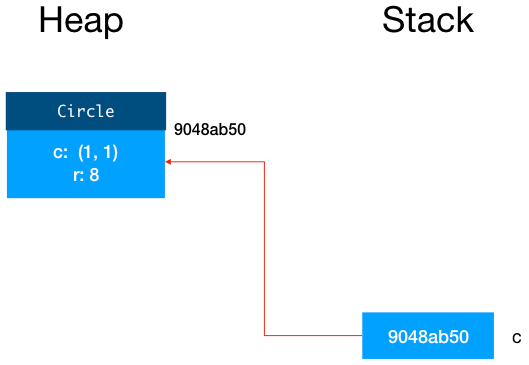
\includegraphics[width=\linewidth]{cs2030-has}
    \captionof{figure}{First Example}
  \end{minipage}
  \begin{minipage}{0.5\linewidth}
    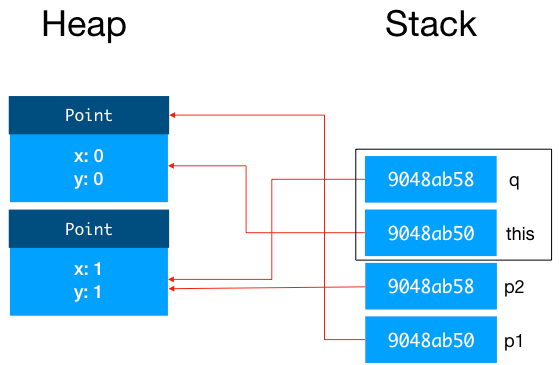
\includegraphics[width=\linewidth]{cs2030-has2}
    \captionof{figure}{Call Stack}
  \end{minipage}
  \subsection{Exceptions}
  \begin{descitemize}
    \item Use \mintinline{Java}{try}/\mintinline{Java}{catch}/\mintinline{Java}{finally} control statements.
  \end{descitemize}
  \begin{minted}[linenos, numbersep=2pt, xleftmargin=3mm]{Java}
try {
  reader = new FileReader(filename);
  scanner = new Scanner(reader);
  numOfPoints = scanner.nextInt();
} catch (FileNotFoundException e) {
  System.err.println("Unable to open " + filename + " " + e);
} catch (InputMismatchException e) {
  System.err.println("Unable to scan for an integer");
} catch (NoSuchElementException e) {
  System.err.println("No input found");
} finally {
  if (scanner != null)
  scanner.close();
}
    \end{minted}
  \begin{descitemize}
    \item Lines 2-4 keep the basic tasks together, lines 12-13 group together all the cleanup tasks
    \item The \mintinline{Java}{finally} block is always executed even when return or throw is called in a \mintinline{Java}{catch} block.
    \item It is also possible to combine multiple catches
  \end{descitemize}
  \begin{minted}{Java}
catch (FileNotFoundException | InputMismatchException | NoSuchElementException e) {
  System.err.println(e);
}
    \end{minted}
  \begin{descitemize}
    \item There are 2 types of exceptions:
    \begin{descitemize}
      \item [Checked exception] is something that the programmer should anticipate and handle.
      \item [Unchecked exception] is something that the programmer does not anticipate, and usually is a result of a bug.
    \end{descitemize}
  \end{descitemize}
  \subsubsection{Checked Exceptions}
  \begin{descitemize}
    \item We need to either catch all checked exceptions or let it propagate to the calling method. Otherwise, the program will not compile.
    \item All methods that throw checked exception need to specify the checked exception(s) using \mintinline{Java}{throws}
  \end{descitemize}
  \begin{minted}[linenos, numbersep=2pt, xleftmargin=3mm]{Java}
public static int readIntFromFile(String filename) throws FileNotFoundException {
  FileReader reader = new FileReader(filename);
  Scanner scanner = new Scanner(reader);
  int numOfPoints = scanner.nextInt();
  scanner.close();
  return numOfPoints;
}
      \end{minted}
  \subsubsection{Generating Exceptions}
  \begin{descitemize}
    \item When you override a method that throws a checked exception, the overriding method must throw only the same, or a more specific checked exception, than the overridden method.
    \item This rule enforces the Liskov Substitution Principle.
  \end{descitemize}
  \begin{minted}{Java}
public Circle(Point p, Point q, double r, boolean centerOnLeft) {
  if (p.distanceTo(q) > 2*r) {
    throw new IllegalArgumentException("Input points are too far apart");
  }
  if (p.equals(q)) {
    throw new IllegalArgumentException("Input points coincide");
}
    \end{minted}
  \subsubsection{Good Practices for Exception Handling}
  \begin{descitemize}
    \item [Catch Exceptions to Clean Up]: It is better to catch the exception, handle the resource deallocation in a \mintinline{Java}{finally} block. If need be, can always re-throw the exception.
  \end{descitemize}
  \begin{minted}{Java}
    public void m2() throws E2 {
      try {
        // Set up resources
      }
      catch (E2 e) {
        throw e;
      }
      finally {
        // clean up resources
      }
    }
    \end{minted}
  \begin{descitemize}
    \item [DO NOT catch all exceptions]:
  \end{descitemize}
  \begin{minted}{Java}
    try {}
    catch (Exception e) {} // NO NO NO NO!!!!
    // Or worse:
    try {}
    catch (Error e) {}     // NO NO NO NO!!!! U WOT M8!!!!
    \end{minted}
  \begin{descitemize}
    \item [Overreacting]: Do not exit just because of exception, especially not silently.
    \item [Do Not Break Abstraction Barrier]: Sometimes, letting the calling method handles the exception causes the implementation details to be leaked, and make it harder to change the implementation later. We should, as much as possible, handle the implementation specific exceptions within the abstraction barrier.
  \end{descitemize}
  \begin{minted}{Java}
    class ClassRoster {
      public Students[] getStudents() throws FileNotFoundException {}
    }
    // Later on
    class ClassRoster {
      public Students[] getStudents() throws SQLException {}
    }
    \end{minted}

  \section{Generics and Collections}
  \subsection{Abstract Class and Interface with Default Methods}
  \begin{descitemize}
    \item [Abstract Class]:
  \end{descitemize}
  \begin{minted}{Java}
    abstract class PaintedShape {
      Color fillColor;
      void fillWith(Color c) {
        fillColor = c;
      }
      abstract double getArea();
      abstract double getPerimeter();
    }
    \end{minted}
  \begin{descitemize}
    \item [Interface with default implementation] (introduced in Java 8): using the keyword \mintinline{Java}{default}
  \end{descitemize}
  \begin{minted}{Java}
    interface Shape {
      public double getArea();
      public double getPerimeter();
      public boolean contains(Point p);
      default public boolean cover(Point p) {
        return contains(p);
      }
    }
    \end{minted}
  \subsection{Generics}
  \begin{descitemize}
    \item Generic typing is a type of polymorphism, also known as \textbf{parametric polymorphism}.
  \end{descitemize}
  \begin{minted}[linenos, numbersep=2pt, xleftmargin=3mm]{Java}
    class Queue<T> {
      private T[] objects;
      public Queue<T>(int size) {}
      public boolean isFull() {}
      public boolean isEmpty() {}
      public void enqueue(T o) {}
      public T dequeue() {}
    }
    Queue<Circle> cq = new Queue<Circle>(10);
    cq.enqueue(new Circle(new Point(0, 0), 10));
    cq.enqueue(new Circle(new Point(1, 1), 5));
    Circle c = cq.dequeue();
    \end{minted}
  \begin{descitemize}
    \item $T$ is a \textbf{type parameter}. In line 9, \texttt{Circle} is passed as the \textbf{type argument} to $T$, creating a \textbf{parameterised type} \texttt{Queue<Circle>}.
    \item Thus, in line 12, we no longer need to cast because \mintinline{Java}{cq.enqueue(new Point(1, 3));} will generate a compile-time error.
  \end{descitemize}
  \subsubsection{Variance of Generic Types}
  \begin{descitemize}
    \item Generics are \textbf{invariant} w.r.t. the type parameter.
    \item [Wildcards]:
    \begin{descitemize}
      \item Subtyping among generic types are achieved through wildcard types \texttt{?}, e.g. this is OK \mintinline{Java}{Queue<?> qc = new Queue<Shape>();}
      \item However, \texttt{?} is not a type, thus we cannot declare a class as such \mintinline{Java}{class Bar<?> {}}
      \item Wildcards can be bounded using keywords \mintinline{Java}{extends} (for covariant) and \mintinline{Java}{super} (for contravariant)
      \begin{itemize}
        \item \mintinline{Java}{Queue<Circle>} and \mintinline{Java}{Queue<Shape>} are both subtypes of \mintinline{Java}{Queue<? extends Shape>}, but not \mintinline{Java}{Queue<Object>}
        \item \mintinline{Java}{Queue<Object>} and \mintinline{Java}{Queue<Shape>} are both subtypes of \mintinline{Java}{Queue<? super Shape>}, but not \mintinline{Java}{Queue<Circle>}
      \end{itemize}
    \end{descitemize}
  \end{descitemize}
  \subsubsection{Type Erasure}
  \begin{itemize}
    \item For backward compatibility. The type argument is erased during compile time, and the type parameter $T$ is replaced with either \texttt{Object} (if unbounded) or the bound (if bounded)
  \end{itemize}
  Impacts:
  \begin{enumerate}
    \item No support for \textbf{generics of primitive types.}
    \item No \textbf{distinction in method signature} for different type parameters:
  \end{enumerate}
  \begin{minted}{Java}
class A {
  void foo(Queue<Circle> c) {}
  void foo(Queue<Point> c) {}
}
// After type erasure
class A {
  void foo(Queue c) {}
  void foo(Queue c) {}
}
        \end{minted}
  \begin{enumerate}
    \setcounter{enumi}{2}
    \item Using \textbf{static methods/fields} become trickier.
  \end{enumerate}
  \begin{minted}[linenos, numbersep=2pt, xleftmargin=3mm]{Java}
class Queue<T> {
  static int x = 1;
  static T y;
  static T foo(T t) {};
}
        \end{minted}
  \begin{itemize}
    \item \texttt{Queue<Circle>} and \texttt{Queue<Point>} are compiled to \texttt{Queue}, so they share the same $x$
    \item Lines 3-4 raise compilation error, since $T$ could be both \texttt{Circle} and \texttt{Point}
  \end{itemize}
  \begin{enumerate}
    \setcounter{enumi}{3}
    \item We \textbf{cannot create an array} of parameterized types. After type erasure, if this were allowed, it would have been possible to add \texttt{Queue<Circle>} to \texttt{Queue<Point>[]} since after type erasure both are \texttt{Queue}
  \end{enumerate}
  \subsubsection{Raw Types}
  \begin{itemize}
    \item       For backward compatibility, Java allows us to use a generic class to be used without the type argument.
  \end{itemize}
  \begin{minted}{Java}
    Queue<Circle> cq = new Queue();
      \end{minted}
  \begin{itemize}
    \item In Java 5 or later, if we just use \texttt{Queue}, we get a \texttt{Queue} of \texttt{Object}. This is called a \texttt{raw type}. Recent Java compilers will warn you if you use a raw type in your code.
  \end{itemize}

  \subsubsection{Wrapper Class}
  \begin{itemize}
    \item Java provides a set of wrapper classes, one for each primitive type: \texttt{Boolean}, \texttt{Byte}, \texttt{Character}, \texttt{Integer}, \texttt{Double}, \texttt{Long}, \texttt{Float}, and \texttt{Short}.
    \item Java 5 introduces \textbf{autoboxing} and \textbf{unboxing}, which creates the wrapper objects automatically (autoboxing) and retrieves its value (unboxing) automatically.
  \end{itemize}
  \begin{minted}{Java}
    Queue<Integer> iq = new Queue<Integer>(10);
    cq.enqueue(4);
    cq.enqueue(8);
    \end{minted}
  \begin{itemize}
    \item Note that enqueue expects an \texttt{Integer} object, but we pass in an \texttt{int}. This would cause the \texttt{int} variable to automatically be boxed (i.e., be wrapped in \texttt{Integer} object) and put onto the call stack of \texttt{enqueue}.
    \item However, all primitive wrapper classes are immutable. Thus, performance penalty when updating (due to allocating memory and garbage collectipm)
  \end{itemize}
  \subsubsection{Generic Methods}
  \begin{itemize}
    \item The scope of the type parameter is limited to only the method itself. In this case,  $X$ (to prevent confusion. Conventionally, $T$ is used instead)
  \end{itemize}
  \begin{minted}[linenos, numbersep=0pt, xleftmargin=3mm]{Java}
    class Queue<T> {
      static <X> X foo(X t) { return t; };
    }
    Queue.<Point>foo(new Point(0, 0));
    Queue.foo(new Point(0, 0));
    \end{minted}
  \begin{itemize}
    \item On line 5, Java compiler uses \textbf{type inference} to determine what $X$ should be.
    \item Also for constructors using the \textbf{diamond operator} \mintinline{Java}{Queue<Point> q = new Queue<>();}
  \end{itemize}

  \subsection{Java Collections}
  \subsubsection{Set and List}
  \begin{itemize}
    \item \texttt{Set<E>} does not allow duplicates (but still does not care about order of elements) -- a \textbf{set}. Useful classes implementation: \texttt{ArrayList}, \texttt{LinkedList}
    \item \texttt{List<E>} allows duplicates and the order of elements matters -- a \textbf{sequence}. Useful classes implementation: \texttt{HashSet}
  \end{itemize}
  \begin{minted}{Java}
   List<String> names = new ArrayList();
   names.add("Cersei");
   names.add("Joffrey");
   names.add(0, "Gregor");
   System.out.println(names.get(1)); // Prints Cersei
   \end{minted}
  \subsubsection{Comparator}
  \begin{itemize}
    \item \texttt{List<E>} interface specifies \mintinline{Java}{default void sort(Comparator<? super E> c)}
    \item Example Comparator class:
  \end{itemize}
  \begin{minted}{Java}
   class NameComparator implements Comparator<String> {
     public int compare(String s1, String s2) {
       return s1.compareTo(s2); // Sorting by lexicographical order
     }
   }
   \end{minted}
  \subsubsection{Map}
  \begin{itemize}
    \item store a unique key, value pair. \texttt{Map<K,V>} is generic with 2 type parameters.
    \item Useful class implementation: \texttt{HashMap}
  \end{itemize}
  \begin{minted}{Java}
   Map<String,Integer> population = new HashMap<String,Integer>();
   population.put("Oldtown",600000);
   population.put("Kings Landing",500000);
   population.put("Lannisport",300000);
   population.get("Kings Landing"); // Returns 500000
   \end{minted}
  \subsubsection{Which one to use?}
  \begin{descitemize}
    \item [HashMap] if you want to keep a (key, value) pair for lookup later.
    \item [HashSet] no duplicates and order is not important. Quick \texttt{contain} check.
    \item [ArrayList] possible duplicates and order is important, and random access is more important than adding/removing.
    \item [LinkedList] possible duplicates and order is important, adding/removing is more important than random access.
    \item [PriorityQueue] Like a queue but order of poll is according to natural ordering
  \end{descitemize}

  \section{Hash Code, Nested Classes, Enum}
  \subsection{Hash Code}
  \begin{itemize}
    \item If \mintinline{Java}{a.equals(b)} then \mintinline{Java}{a.hashCode() == b.hashCode()} (not necessarily the converse)
    \item How to create \texttt{hashCode()}:
  \end{itemize}
  \begin{minted}{Java}
   class A {
     public double x, y;
     @Override
     public int hashCode() {
       return Arrays.hashCode(new double[] {this.x, this.y});
     }
   }
   \end{minted}
  \begin{itemize}
    \item If you have fields in a class of different types, pack them into different arrays, call \mintinline{Java}{Arrays.hashCode()} for each of the arrays, and combine the hash code together with the XOR operator \texttt{\^}
  \end{itemize}
  \subsection{Nested Class}
  \begin{itemize}
    \item A nested class can be either \textbf{static} or \textbf{non-static}.
    \item A \textbf{static nested class} is associated with the containing class, NOT an instance. So, it can only access static fields and static methods of the containing class.
    \item A \textbf{non-static nested class} can access all fields and methods of the containing class. A non-static nested class is also known as an \textbf{inner class}.
  \end{itemize}
  \subsubsection{Local Class}
  \begin{itemize}
    \item Classes that are declared inside a method (more precisely, inside a block of code between \{ and \}) is called a \textbf{local class}.
    \item A local class is scoped within the method. It has access to the variables of the enclosing class and local variables of the enclosing method.
  \end{itemize}
  \begin{minted}{Java}
   void sortNames(List<String> names) {
     class NameComparator implements Comparator<String> {
       public int compare(String s1, String s2) {
         return s1.length() - s2.length();
       }
     }
     names.sort(new NameComparator());
   }
   \end{minted}
  \subsubsection{Variable Capture}
  \begin{itemize}
    \item A local class \textbf{captures} the local variables in the enclosing method (the local class makes a copy of local variables in the enclosing method inside itself.).
  \end{itemize}
  \subsubsection{Effectively final}
  \begin{itemize}
    \item Java only allows a local class to access variables that are explicitly declared final or implicitly final (or effectively final).
    \item An implicitly final variable is one that does not change after initialization.
  \end{itemize}
  \subsubsection{Anonymous Class}
  Format: \texttt{new X (arguments)\{ body \}}
  \begin{itemize}
    \item \textbf{X} is a class that the anonymous class extends or an interface that the anonymous class implements. (cannot be empty, no multiple inheritance -- cannot extend a class and implement an interface, cannot implement more than one interface)
    \item \textbf{arguments} are the arguments that you want to pass into the constructor of the anonymous class. (If extending an interface, there is no constructor, but we still need \texttt{()})
    \item \textbf{body} the body of the class as per normal, except that we cannot have a constructor.
  \end{itemize}
  \begin{minted}{Java}
   names.sort(new Comparator<String>() {
     public int compare(String s1, String s2) {
       return s1.length() - s2.length();
     }
   });
   // OR
   Comparator<String> cmp = new Comparator<String>() {
     public int compare(String s1, String s2) {
       return s1.length() - s2.length();
     }
   };
   names.sort(cmp);
   \end{minted}
  \begin{itemize}
    \item The same rules to variable access as local class applies.
  \end{itemize}

  \subsection{Enum}
  \begin{itemize}
    \item Variable of an enum type can only be one of the predefined constants.
    \item Trying to assign anything other than the two predefined event type to eventType would result in compilation error.
  \end{itemize}
  \begin{minted}{Java}
   enum EventType {
     CUSTOMER_ARRIVE,
     CUSTOMER_DONE
   }
   class Event {
     private double time;
     private EventType eventType;
   }
   \end{minted}
  \subsubsection{Enum's Fields and Methods}
  \begin{itemize}
    \item Each constant of an enum type is actually an instance of the enum class and is a field in the enum class declared with \mintinline{Java}{public static final}.
    \item Since enum in Java is a class, we can define constructors, methods, and fields in enums.
  \end{itemize}
  \begin{minted}{Java}
    enum Color {
      BLACK(0, 0, 0),
      WHITE(1, 1, 1),
      RED(1, 0, 0),
      BLUE(0, 0, 1),
      GREEN(0, 1, 0),
      YELLOW(1, 1, 0),
      PURPLE(1, 0, 1);
      private final double r;
      private final double g;
      private final double b;
      Color(double r, double g, double b) {
        this.r = r;
        this.g = g;
        this.b = b;
      }
      public double luminance() {
        return (0.2126 * r) + (0.7152 * g) + (0.0722 * b);
      }
      public String toString() {
        return "(" + r + ", " + g + ", " + b + ")";
      }
    }
    Color a = Color.YELLOW;
    System.out.println(a); // Prints (1.0, 1.0, 0.0)
    a.luminance(); // Returns 0.9278
    \end{minted}
  \subsubsection{Custom Methods for Each Enum}
  \begin{itemize}
    \item We can define custom methods for each of the enum constant, by writing constant-specific class body.
  \end{itemize}
  \begin{minted}{Java}
    enum EventType {
      CUSTOMER_ARRIVE {
        void log(double time, Customer c) {
          System.out.println(time + " " + c + " arrives");
        }
      },
      CUSTOMER_DONE {
        void log(double time, Customer c) {
          System.out.println(time + " " + c + " done");
        }
      };
      abstract void log(double time, Customer c);
    }
    EventType.CUSTOMER_DONE.log(time, customer);
    \end{minted}
  \subsubsection{The Class Enum}
  \begin{itemize}
    \item All \texttt{enum} inherits from the class \texttt{Enum} implicitly.
  \end{itemize}
  \begin{minted}{Java}
    // The example in 6.3 is actually
    public final class EventType extends Enum<EventType> {
      public static final EventType[] values { .. }
      public static EventType valueOf(String name) { .. }

      public static final EventType CUSTOMER_ARRIVE;
      public static final EventType CUSTOMER_DONE;
      :

      static {
        CUSTOMER_ARRIVE = new EventType();
        CUSTOMER_DONE = new EventType();
        :
      }
    }

    \end{minted}

  \begin{itemize}
    \item To ensure that the generic type \texttt{E} actually inherits from \texttt{Enum<E>}, class Enum is defined to be generic type \mintinline{Java}{Enum<E extends Enum<E>>}
    \item An \texttt{enum} is final. We cannot inherit from enum (those with constant-specific body are exceptions).
    \item A class in Java can contain fields of the same class.
    \item The block marked by static { .. } are static initializers, they are called when the class is first used. They are the counterpart to constructors for objects, and are useful for non-trivial initialization of static fields in a class.
    \item Two useful classes \texttt{EnumSet} and \texttt{EnumMap} -- special cases of \texttt{HashSet} and \texttt{HashMap} respectively -- the only difference is that we can only put enum values into EnumSet and enum-type keys into EnumMap.

  \end{itemize}


  \section{Functions}
  \subsection{Pure Functions}
  \begin{itemize}
    \item \textbf{No side effect} (including but not limited to printing to the screen, writing to files, throwing exceptions, changing other variables, modifying the values of the arguments.)
    \item \textbf{Deterministic} (given same input, produces same output everytime)
  \end{itemize}
  \subsection{\texttt{Function} interface and other related interfaces in Java 8}
  \begin{tabular}{|l|l|}
    \hline
    Interface                              & SAM                                  \\ \hline
    \mintinline{Java}{Function<T, R>}      & \mintinline{Java}{R apply(T t)}      \\
    \mintinline{Java}{Supplier<T>}         & \mintinline{Java}{T get()}           \\
    \mintinline{Java}{Consumer<T>}         & \mintinline{Java}{void accept(T t)}  \\
    \mintinline{Java}{BiFunction<T, U, R>} & \mintinline{Java}{R apply(T t, U u)} \\
    \hline
  \end{tabular}
  \subsection{Lambda Expression}
  \begin{minted}{Java}
// All are equivalent
applyList(list, new Function<Integer,Integer>() {
  public Integer apply(Integer x) {
    return x * x;
  }
});
applyList(list, (Integer x) -> { return x * x; });
applyList(list, x -> { return x * x; });
applyList(list, x -> x * x);

// Method Reference
applyList(list, x -> Math.abs(x));
applyList(list, Math::abs);
    \end{minted}
  \subsection{Composing Functions}
  \mintinline{Java}{default <V> Function<T,V> andThen(Function<? super R,? extends V> after);}\\
  \mintinline{Java}{default <V> Function<V,R> compose(Function<? super V,? extends T> before);}
  \begin{minted}{Java}
Function<Integer,Integer> abs = Math::abs;
Function<Integer,Double> sqrt = Math::sqrt;
// All are equivalent
x -> Math.sqrt(Math.abs(x));
abs.andThen(sqrt));
sqrt.compose(abs));
    \end{minted}

  \subsection{PECS}
  \mintinline{Java}{default <V> Function<T,V> andThen(Function<? super R,? extends V> after);}\\

  We can make the method more general by allowing it to take a function with R or any superclass of R as input -- \textbf{surely if the function can take in a superclass of R, it can take in R}. Thus, we can relax input type, or what the function consumes, from R to ? super R.\\

  Similarly, if we are expecting the function after to return a more general type V, \textbf{it is fine if it returns V or a subclass of V}. Thus, we can relax the return type, or what the function produces, from V to ? extends V.\\

  mnemonic "producer extends; consumer super", or PECS, for short.


  \section{Streams}
  \subsection{Lambda as Closure}
  \begin{itemize}
    \item A lambda expression can capture the variables of the enclosing scope since lambda expression is just a shorthand to an anonymous class.
    \item A captured variable must be either explicitly declared as final or is effectively final.
  \end{itemize}
  \subsection{\texttt{Optional<T>} class}
  \subsection{\texttt{Stream} class}

  \section{FP Patterns}
  \begin{minted}{Java}
interface Thing<T> {
  public <R> Functor<R> f(Function<T,R> func);
  public <R> Monad<R> f(Function<T, Thing<R>> func);
}
      \end{minted}
  \subsection{Functor}
  \begin{itemize}
    \item It will "unwrap" the value, applies the function, then re-"wrap" the value.
    \item e.g. \texttt{Optional} class.
  \end{itemize}
  \subsection{Functor Laws}
  \begin{itemize}
    \item if \texttt{func} is an identity function \mintinline{Java}{x -> x}, then it should not change the functor.
    \item if \texttt{func} is a composition of two functions $g\cdot h$, then the resulting functor should be the same as calling $f$ with $h$ and then with $g$.
  \end{itemize}
  \subsection{Monad}
  \begin{itemize}
    \item It will "unwrap" the value, applies the function which returns an already wrapped value.
    \item e.g. \texttt{Stream} class
  \end{itemize}
  \subsection{Monad Laws}
  \begin{itemize}
    \item $\exists$ an \texttt{of} operation that takes (an) object(s) and wrap it / them into a monad:
          \begin{itemize}
            \item \textbf{Left identity law}: \texttt{Monad.of(x).flatMap(f) == f(x)}
            \item \textbf{Right identity law}: \texttt{monad.flatMap(x -> Monad.of(x)) == monad}
          \end{itemize}
    \item \textbf{Associative law}: the \texttt{flatMap} operation should be associative -- \texttt{monad.flatMap(f).flatMap(g) == monad.flatMap(x -> f(x).flatMap(g))}
  \end{itemize}
  \subsection{Implementing Strategy / Policy}
  \begin{itemize}
    \item OO using polymorphism through inheritance.
    \item FP using \texttt{Runnable}
  \end{itemize}
  \subsection{Observer Pattern}
  Basically event-driven: add actions to do when triggerred.

  \section{Parallel Streams}
  By adding \texttt{parallel()} anywhere in the chain, e.g.:
  \begin{minted}{Java}
IntStream.range(2_030_000, 2_040_000)
    .filter(x -> isPrime(x))
    .parallel()
    .forEach(System.out::println);
    \end{minted}
  \subsection{Ensuring correctness of parallelisation}
  Criteria:
  \begin{itemize}
    \item \textbf{No interference}: stream operations must not modify the source of the stream during execution.
    \item \textbf{Stateless}: stream operations must not depend on any external state that might change during execution.
    \item \textbf{No side effects}
    \item \textbf{Associativity}: For \texttt{reduce}:
          \begin{itemize}
            \item \texttt{combiner.apply(identity, i) == i}
            \item The combiner and the accumulator must be associative -- the order of applying must not matter.
            \item The combiner and the accumulator must be compatible -- \\ \texttt{combiner.apply(u, accumulator.apply(identity, t)) == accumulator.apply(u, t)}
          \end{itemize}
  \end{itemize}
  \begin{minted}{Java}
// Associativity Example:
Stream.of(1,2,3,4).reduce(1, (x,y)->x*y, (x,y)->x*y);
// i * 1 == i
// (x * y) * z == x * (y * z)
// u * (1 * t) == u * t

// Using non-thread-safe data structure:
List<Integer> result =
    list.parallelStream()
        .filter(x -> isPrime(x))
        .collect(Collectors.toList())
// Or using a thread-safe data structure
List<Integer> result = new CopyOnWriteArrayList<>();
list.parallelStream()
  .filter(x -> isPrime(x))
  .forEach(x -> result.add(x));
    \end{minted}

  \subsection{Fork and Join}
  \begin{itemize}
    \item \texttt{ForkJoinTask<V>} abstract class has 2 important methods \texttt{fork()} (submits task for execution) and \texttt{join()} (waits for computation to complete and returns the value)
    \item \texttt{RecursiveTask<V>} abstract class is a subclass of \texttt{ForkJoinTask<V>} with a method \texttt{V compute()}
  \end{itemize}

  \section{Asynchronous}
  \subsection{\texttt{Future<T>} Interface}
  Implemented by both \texttt{RecursiveTask} and \texttt{RecursiveAction}. Five simple operations:
  \begin{itemize}
    \item \texttt{get()} result of computation (waiting if needed)
    \item \texttt{get(timeout, unit)} same but waiting up to timeout period
    \item \texttt{cancel(interrupt)}
    \item \texttt{isCancelled()}
    \item \texttt{isDone()}
  \end{itemize}
  \subsection{\texttt{CompletableFuture<T>} interface}


  %   \begin{minted}{javascript}

  %   \end{minted}
\end{multicols*}
\end{document}
